\subsection{Simulating neural activity in a neural population} \label{sec:results:simulations}

To test the described method for inferring functional connectivity from calcium imaging data, we simulated networks of stochastically connected neurons, simulated according to our model, Eqs \ref{eqn:glm:definition} -- \ref{eqn:F:definition}.  Simulations ran at $1$ msec time discretization, although we assumed that we made observations intermittently (i.e., not every time step). Model parameters were chosen based on experimental data available from the literature \cite{Braitenberg1998, Urquijo2000, Lefort2009, Sayer1990}.  

More specifically, the network was divided into excitatory (80\%) and inhibitory (20\%) neurons \cite{Braitenberg1998, Urquijo2000}, each respecting Dale's law, i.e., each neurons was either excitatory or inhibitory (corresponding to all positive or all negative columns in our functional connection weight matrix, $\bw$). Neurons were randomly connected to each other with probability $0.1$ \cite{Braitenberg1998, Lefort2009}. Synaptic weights for excitatory connections, as defined by EPSP peak amplitude, were randomly drawn from exponential distribution with the mean of $0.5 \mu V$ \cite{Lefort2009, Sayer1990}. These were then converted to functional connectivity weights: while synaptic weights physiologically were measured in $\mu V$, in our model, functional connectivity weights were measured in log-rate units of Eq. \ref{eqn:glm:definition}). Thus, functional connectivity weights describe the change in the probability of the neuron $i$ firing, given neuron $j$ fired, as opposed to physiologically measured injected currents or changes in membrane potential. Figure \ref{fig:fr_vs_J} explicitly depicts this relationship, for our model.  Note that a spike in a presynaptic neuron changes $J$ by $w_{ij}h_j(t)$. By utilizing this definition, synaptic weights were converted into functional connectivity weights assuming that each EPSP corresponded to added probability of neuron spiking in given time bin of $\Delta P = V_E/V_{\delta}$, where $V_E$ is peak EPSP amplitude and $V_{\delta}$ is the difference between the neuron's resting potential and threshold (implying that $V_{\delta}/V_E$ EPSPs would be required to trigger neuron over the threshold):

\begin{equation}\label{eqn:convert}
\w_{ij}=\ln(-\ln(e^{-r_i\tau_w}-V_E/V_{\delta})/r_i\tau_w),
\end{equation}

\noindent where $r_i=\exp(b_i)$ is the base firing rate of neuron $i$ and $\tau_w=10$ msec was the typical EPSP/IPSP scale over which single EPSP affects the firing probability of the neuron $i$.  %For small $r_i\tau_w$ this could be replaced with
%
% \begin{equation}\label{eqn:convert-smalldt}
% \w_{ij}=\ln\left(1+\frac{V_E/V_{\delta}}{r_i\tau_w}\right).
% \end{equation}

Inhibitory connections were also drawn from exponential distribution, with negative magnitudes imposed, and their strengths chosen so as to balance excitatory and inhibitory currents in the network and achieve an average firing rate of  $\approx 5 $ Hz. Practically, the mean strength of inhibitory connections was about 10 times larger than that of the excitatory connections.

XXX this sentence might need work depending on what liam decides about $w_{ij}(t)$ vs $h_j(t)$. XXX The time course of functional connectivity weights $\w_{ij}(t)$ was modeled as the difference of two exponentials, resulting in a rise time of $\tau_r=1$ msec and decay time of $\tau_{E_d}=10$ msec for excitatory and $\tau_{I_d}=20$ msec for inhibitory currents \cite{Sayer1990}. In practice, we sampled time constants from uniform distributions with means as stated above and support of $\pm 25 \%$ of the means. We neglected conduction delays, given that the time delay below $\sim 1$ msec expected in local cortical circuit was smaller than the time step of our computer simulation.  Each neuron also had an exponential refractory current with a $10$ msec time constant. XXX Y: did that not get sampled? XXX

Parameters for the calcium dynamics and observation statistics were chosen according to our experience with several cells analyzed using algorithm of \cite{Vogelstein2009}, see Table \ref{table:caparm}.  The population of cells was generated with these parameters allowing cell-to-cell variance of at least 30\%. More specifically, each parameter was generated from a normal distribution with specified mean and variance at about 30\% of the mean, truncated at the lower bound at about 30\% of the mean value. Fluorescence was obtained for calcium imaging at the frame rate of 33 Hz or 66 Hz.  From 5 to 60 minutes of calcium imaging data was simulated.

\begin{table}[h!b!p!]
\caption{Table of simulation parameters.}\label{table:caparm}
\begin{tabular}{ll}
\hline
Total neurons & 10-500 \\
Excitatory neurons & 80\% \\
Connections sparseness & 10\% \\
Baseline firing rate & 5  Hz\\
Mean EPSP strength & (0.5 $\mu$V) \\
Mean IPSP strength & 2.3 $\mu$V\\
EPSP profile & 1 msec rise time, 10 msec decay time \\
IPSP profile & 1 msec rise, 20 msec decay time \\
\hline
Mean Ca noise $\sigma_c$ & 28 $\mu$M \\
Mean Ca jump $A_c$ & 80 $\mu$M \\
Mean Ca background $C_b$ & 24 $\mu$M \\
Mean Ca decay time $\tau_c$ & 0.25 sec \\
Mean photon budget $\alpha_c$ & 1-80 Kph/neuron/frame \\
$K_d$ & 200 $\mu$M \\
\hline
\end{tabular}
\end{table}


\begin{figure}[h]
\centering 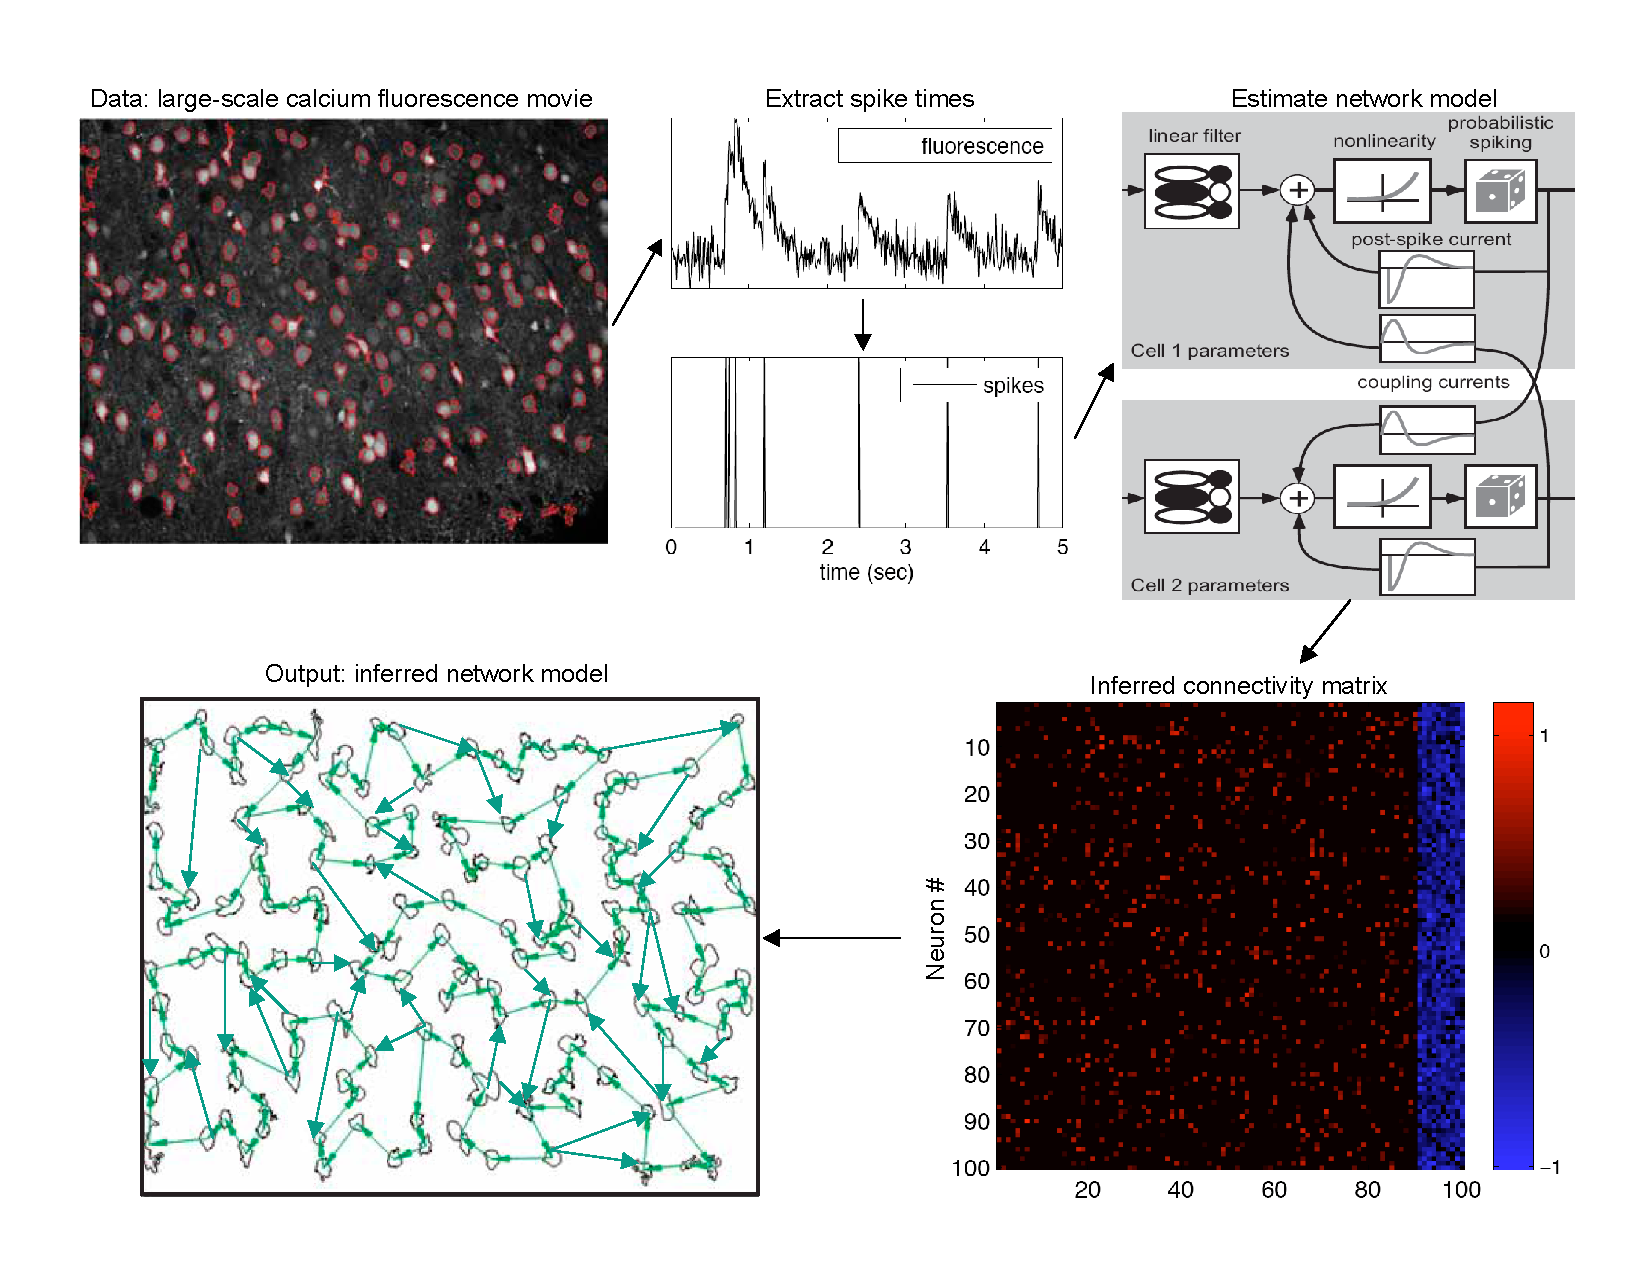
\includegraphics[width=\hsize]{../figs/yuri-paper-schematic}
\caption{Schematic overview. First we obtain large-scale calcium recordings of spontaneous 
and evoked neural responses.  These movies are then pre-processed to correct for movement artifacts, find regions-of-interest, and extract spike trains.  Second, given the fluorescence traces from each neuron, we infer spike trains.  Third, we use our population model to infer the most likely functional connectivity matrix, which is our approximation of the microcircuit.}
\label{fig:egfluor}
\end{figure}


\subsection{Inferring functional connectivity from the simulated calcium imaging data} \label{sec:results:inference}

%Fig 1: data example
%left: imagesc of real data
%right top: neuron with high SNR
%right bottom: neuron with low SNR
%
%Fig 2: connection weight example
%left: true w matrix
%right: estimated w matrix
%-------------------------------------------------------------------------------------------

With neural population activity prepared as described in the previous section,
we used our Bayesian inference algorithm to reconstruct the functional connectivity matrix from simulated fluorescence data.
Specifically, we calculated the connectivity matrix by solving the maximum likelihood problem Eq. \ref{eqn:likelihoodGLM-expl},
\begin{align}
\label{eqn:likelihoodGLMmoda}&E[\ln P_{\bn}(n_i|{\bf n}_{\i}; W)]=\sum_t \left( n_i(t) \ln J_i(t) - (1-n_i(t)) \exp(J_i(t)) \Delta \right), \\
\label{eqn:likelihoodGLMmodb}&J_i(t)=b_i+\sum\limits_j \sum\limits_{t'<t} \w_{ij}(t-t')n_{j}(t')=
b_i+\sum\limits_j w_{ij} h_j(t).
\end{align}
The sum in Eqs.\ref{eqn:likelihoodGLMmoda} and \ref{eqn:likelihoodGLMmodb} was over the sample of $\{n_i(t)\}$, produced with our spike sampling algorithm, discretized over the time-bins $t'$ with the width corresponding to the calcium imaging frame rate (i.e. 30 ms for 33 Hz and 15 ms for 66 Hz). In one of the two cases we considered, EPSP time-profiles were assumed to be ``known'' exponential, and the weights were estimated using reduced histories $h_{i}(t)=\sum_{t'<t} \exp(-(t-t')/\tau_h)n_{i}(t')$ with the time constant $\tau_h=10$ ms (i.e. second equation in Eq. \ref{eqn:likelihoodGLMmodb}). In the second case we considered, the time dependence of $\w_{ij}(t)$ was assumed to be unknown and the first equation in Eq. \ref{eqn:likelihoodGLMmodb}) was used to correlate $n_i(t)$ with $n_j(t')$ for $t'<t$ up to a given depth $m$.  In this latter case, since each next term in Eq. \ref{eqn:likelihoodGLMmodb}) was significantly smaller than the previous one, we found that the best results were obtained if we took $m=1$ (i.e. minimizing number of unknown variables given certain amount of data).
In either case, we described the connection weight between two neurons by a scalar quantity $w_{ij}^s=\text{sign}(\w_{ij})\max_{t} |\w_{ij}(t)|$, which thereafter was used to compare true and reconstructed connectivity weights in all examples below.

%Fig 3: gibbs, indep, baseline results
%left: uncorrected scatter plot
%middle: corrected (theory or actual to be decided later) scatter plot
%right:  gibbs, indep, baseline, and true distribution of weights (if this looks too messy, then maybe one subfig for %each case)
\begin{figure}[h]
\centering
\begin{minipage}[c]{0.45\hsize}
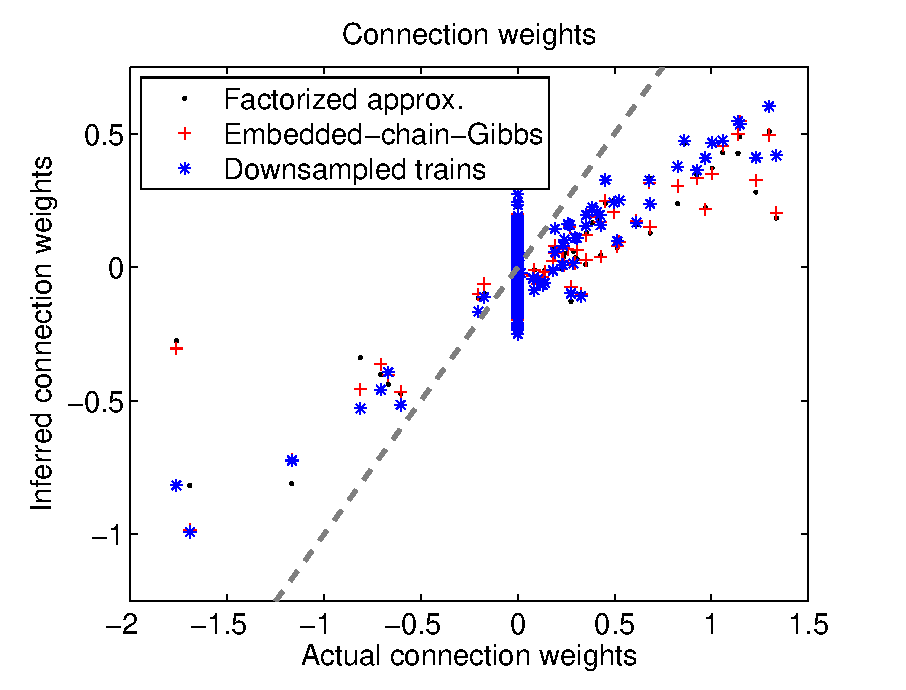
\includegraphics[width=\hsize]{../figs/FigureA3_scatter_three}
\end{minipage}
\begin{minipage}[c]{0.45\hsize}
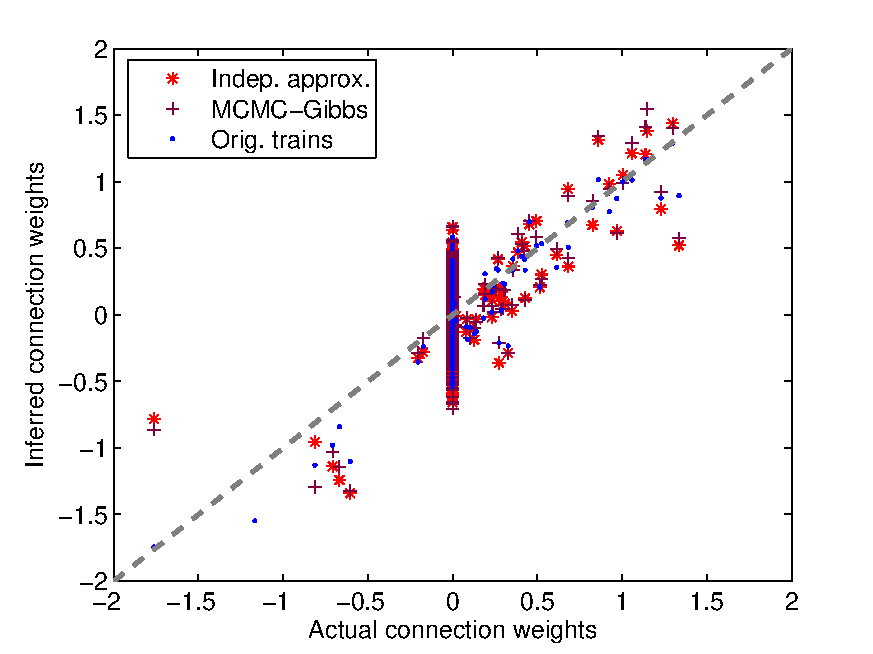
\includegraphics[width=\hsize]{../figs/FigureA3_scatter_three_corrected}
\end{minipage}
% \begin{minipage}[c]{0.3\hsize}
% 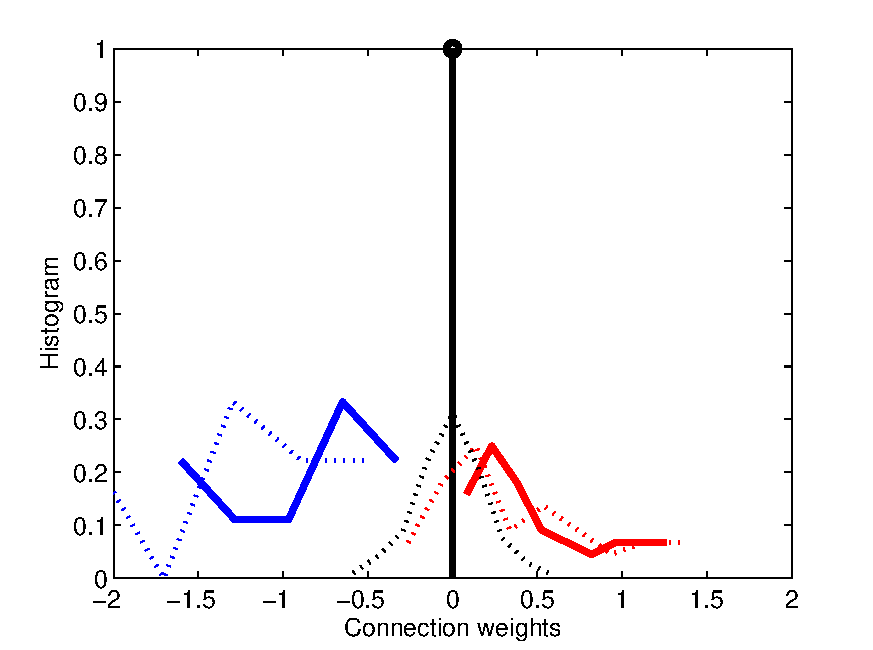
\includegraphics[width=\hsize]{../figs/FigureA3_hist_iid}
% \end{minipage}
% \begin{minipage}[c]{0.3\hsize}
% 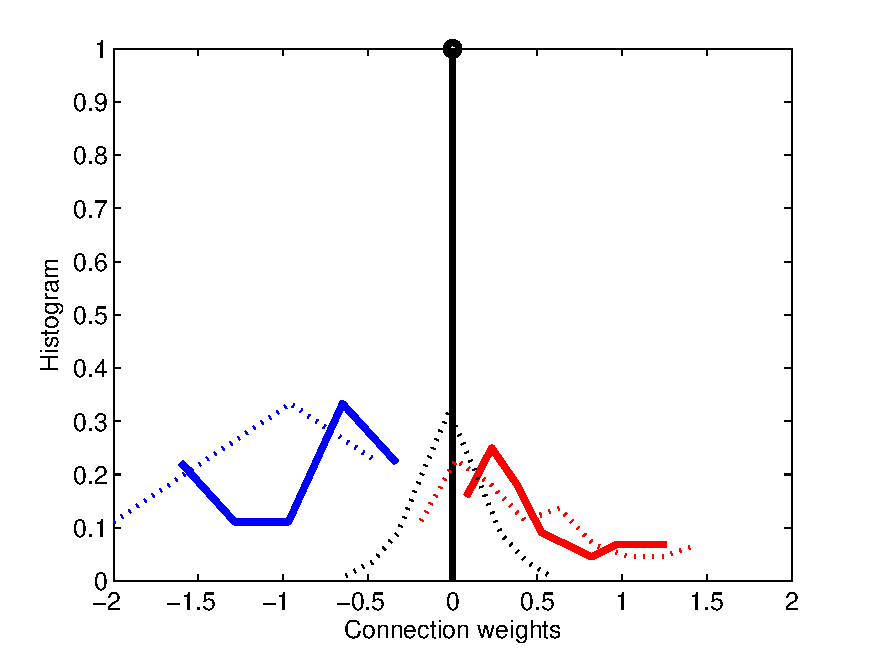
\includegraphics[width=\hsize]{../figs/FigureA3_hist_mcmc}
% \end{minipage}
% \begin{minipage}[c]{0.3\hsize}
% 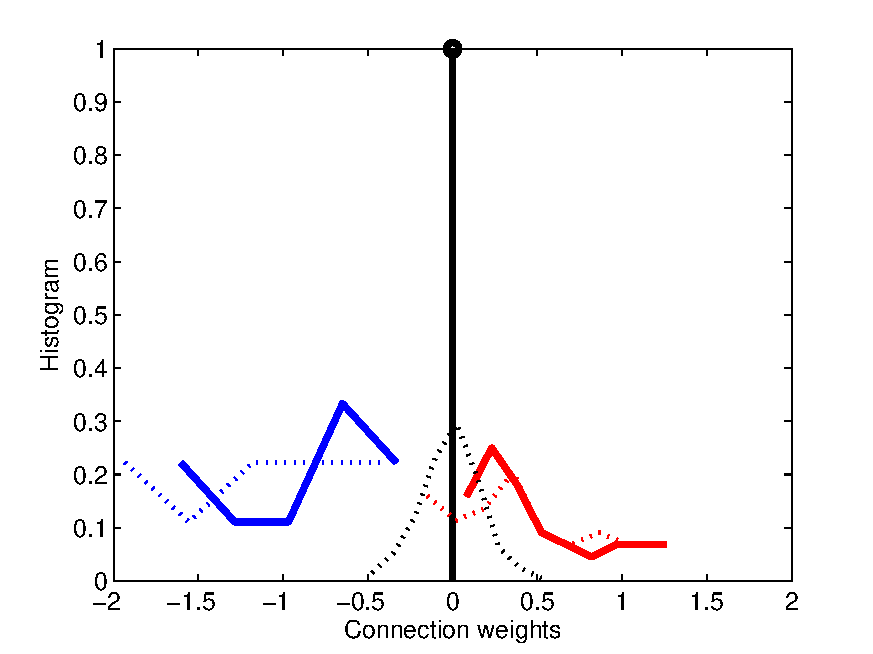
\includegraphics[width=\hsize]{../figs/FigureA3_hist_orig}
% \end{minipage}
\caption{Functional connectivity matrix can be reconstructed from calcium imaging data.
In the upper panels inferred connection weights are shown in a scatter plot versus real connection weights, with inference performed using independent approximation algorithm, exact MCMC-Gibbs algorithm, and original spike trains observed at the frame rate of the calcium imaging. Network of $N=25$ neurons was used, firing at $\approx 5$ Hz, and imaged for T=600 sec at intermediate SNR (photon budget 10Kph/neuron/frame, see below).
$r^2=0.47$ for independent approximation algorithm was found, $r^2=0.48$ for MCMC-Gibbs algorithm, and $r^2=0.57$ for the original spike trains.
Thus, independent approximation produced results almost as accurate as the exact MCMC-Gibbs algorithm, and almost as accurate as the original spikes.
Inferred connectivity weights (upper left) were scaled with respect to true connectivity by a constant amount due to time discretization bias (see below); other than scale, inferred connectivity represented the true connectivity matrix very well (upper right).
% Lower panels show the inferred histograms of the connection weights (dotted lines) versus that of the true connectivity matrix (think solid lines). Blue corresponds to negative (inhibitory) connections, red corresponds to positive (excitatory) connections, and black corresponds to zero (absent) connections in the true connectivity matrix.
Thus, calcium imaging is sufficient to identify connected pairs of neurons reliably.}
\label{fig:scatters}
\end{figure}


We performed reconstruction of functional connectivity from fluorescence data using MCMC-Gibbs algorithm as well as using independent approximation, Figure \ref{fig:scatters}. We found that independent approximation algorithm was able to provide reconstructions almost as accurate as the exact MCMC-Gibbs algorithm for experimentally interesting imaging regimes. We therefore concluded that the independent approximation was essentially equivalent to the exact MCMC-Gibbs method for the purpose of functional connectivity reconstruction.

We then performed reconstruction of functional connectivity from the original (true) spike trains down-sampled at the frame rates of calcium imaging.
Fluorescence data is generally acquired at low frame rate and, so, one of its main limitations is bad time-resolution of the observed spike trains. To determine the impact of this constraint on the connectivity reconstructions, and, thus, to determine how close calcium imaging may approach  reconstructions from spike trains directly observed under comparable conditions, we conducted this experiment.
We observed that at intermediate SNR reconstructions from calcium imaging closely resembled such obtained directly from spike trains, and at higher SNR reconstruction with the quality same with original spike trains was achieved, Figure \ref{fig:scatters} and \ref{fig:recvar-SNR}.

\subsection{Scale bias in inferred connection weights due to coarse time discretization of calcium imaging data}

Our estimated connectivity matrix was always scaled with respect to the true connectivity by a constant factor. The origin of this bias is the time discretization of the spike trains inferred from calcium imaging, $\Delta \approx 15-30$ ms, large relative to EPSP/IPSP time scale $\tau_w = 10-20$ ms. Really, if $\Delta$ is large, the first term in the sum Eq. \ref{eqn:likelihoodGLMmodb}, $\w_{ij}(\Delta)\approx w_{ij}^s\exp(-\Delta/\tau_w)$, is substantially smaller than $w_{ij}^s$, and the connectivity weights $w_{ji}(\Delta)$ estimated from GLM will be smaller than the true $w^s_{ij}$.

Specifically, to estimate the magnitude of this scale bias consider two neurons coupled with each other via GLM weight $w_{12}$. Assume that, aside from this coupling, these neurons fire with baseline firing rate of $r=\exp(b)$, $b \gg w_{12}$.
In order to estimate $w_{12}$ we observe the number of spike-pairs such that the first neuron fired after the second neuron over some small period of time $\tau_w \ll T \ll 1/r$, which is in excess of the baseline firing rate
$\Delta n(2\rightarrow 1) = n(2\rightarrow 1) - r T \approx \int dt w_{12} \exp(-t/\tau_w)$.

Now, assume that spike trains were additionally discretized into time-bins of size $\Delta$ and only the spikes that occurred in different time-bins were considered as non-coincidental.
In this case, the number of spike-pairs such that the spike of the first neuron followed that of the second neuron observed empirically is $\Delta n'(2\rightarrow 1) \approx \int\limits_0^\Delta {dt_1}/{\Delta} \int\limits_{\Delta}^T dt_2 \exp(-(t_2-t_1)/\tau_w)$. The ratio of the empirical count, $\Delta n'(2\rightarrow 1)$, to that expected from GLM for given $w_{12}$, $\Delta n(2\rightarrow 1)$, is the scale bias that we observe in Figure \ref{fig:scatters},
\begin{equation}\label{eqn:bias}
\Delta n'_{12}/\Delta n_{12}\approx (1-\exp(-\Delta/\tau_w))/(\Delta/\tau_w).
\end{equation}

In Figure \ref{fig:bias} we plotted this estimated magnitude versus that empirically observed from our simulations for different values of $\Delta$. As can be seen from Figure \ref{fig:bias}, simple theoretical estimate Eq.(\ref{eqn:bias}) described observed scale bias quite well.

%Fig 4:  time discretization error (i still think errorbars are necessary for this plot.  for instance, consider the %point at zero discretization error.  the actual bias ~=1, although it clearly should (and does, by definition).  this %leads me to wonder how accurate the theory is.
\begin{figure}[h]
\centering
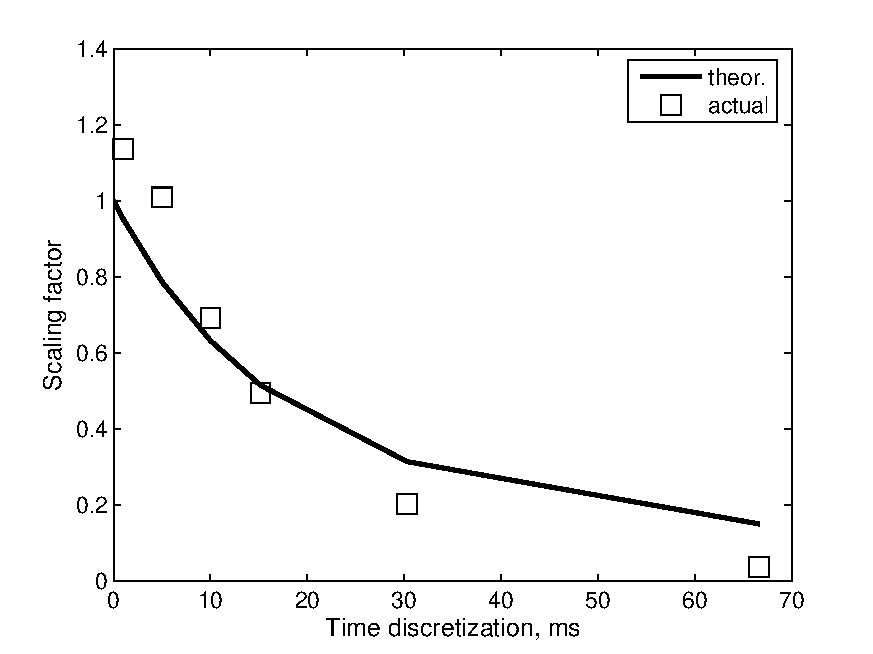
\includegraphics[width=3in]{../figs/FigureA4_scale_bias}
\caption{Low-frame rate of calcium imaging, leading to large bin size $\Delta\approx 15-30$ ms of the inferred spike trains, is the reason of scale bias in the estimated connectivity matrix.
This bias is explained by considering what number of causally-related spikes from
a pair of neurons occur within the same time-bin for bin size $\Delta$, and so are not considered as causally related but coincidental in the time-discretized spike trains.}
\label{fig:bias}
\end{figure}

Scale bias in principle may be removed by performing inference of the spike trains with the bin size $\Delta \rightarrow 0$.
However, we were not successful in performing this calculation.
One problem that we encountered with this approach was the increase in the variance of the connectivity estimates.
In Eq.(\ref{eqn:likelihoodGLMmodb}) the coincident time bin $t=t'$ was omitted from the sum and so all spike pairs within the same time-bins were removed from the GLM fit.  Because time position of such spike pairs inferred from fluorescence data typically would have inaccuracy $\approx \Delta$, temporal order of such spike pairs could often be confused, introducing ambiguity as to whether observed event should contribute to $w_{ij}$ or $w_{ji}$. 

Really, if the number of spikes of one neuron following that of another neuron within $\Delta$ was $n(2\rightarrow 1)$, while such in the reverse order was $n(1\rightarrow 2)$, difference $\delta n_{12} = n(2\rightarrow 1)-n(1\rightarrow 2)$ would correspond to the difference of functional connectivity weights $\delta w_{12}=w_{12}-w_{21}$. However, when such spike pairs had had their order confused with large probability $p\approx 1/2$, the number of spike pairs $n(2\rightarrow 1)$ actually observed would become $(1-p) n(2\rightarrow 1)+p n(1\rightarrow 2)$, and similarly for the reverse. Empirically observed difference $w_{12}-w_{21}$ thus would correspondingly drop to $\delta w'_{12}= (1-2p)\delta w_{12}$, while the variance would remain the same. This effect complicated estimating of the functional connectivity matrix $W$ by effectively mixing $\w_{12}$ and $\w_{21}$ and introducing large error in $W$ estimates, moving them toward $(W+W^T)/2$.
We observed that the amount of data necessary to overcome this noise due to disordering of closely positioned spike-pairs appeared to be well over $\approx 10$ min of data used for the most of the calculations shown in this section below. Such high-time-resolution samples of spike trains also were substantially more computationally expensive to obtain and work with. For these reasons, we did not pursue this line of research further, although it may be of interest in the future.

\subsection{Impact of different imaging frame rates, durations, and noise levels on the inference}
%Fig -: r^2 vs frame rate for T=600 sec
%
%Fig 5: r^2 vs. SNR for various FR
%
%Fig 6:  r^2 vs. T for various N (both naive and sparse)
%
\begin{figure}[h]
\centering
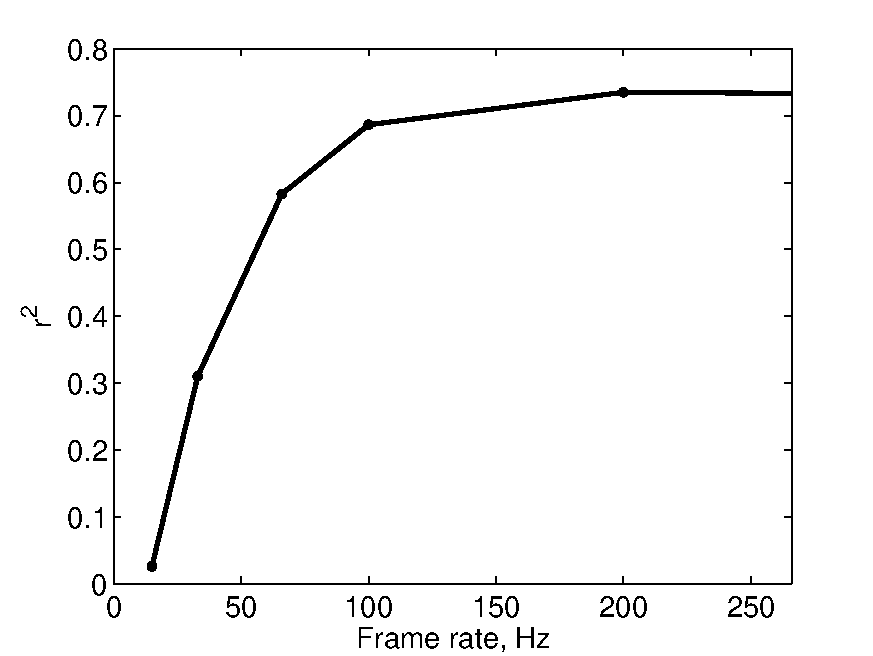
\includegraphics[width=3in]{../figs/FigureA5_recvar}
\caption{Accuracy of the inferred connectivity weights as function of the frame rate of calcium imaging. Connectivity matrix here was inferred from the original spike trains observed at corresponding frame rates, thus establishing the upper performance bound for inference using calcium imaging data. A network of $N=25$ neurons, firing at $\approx 5$ Hz and imaged for $T=600$ sec was used.}
\label{fig:recvar}
\end{figure}

\begin{figure}[h]
\centering
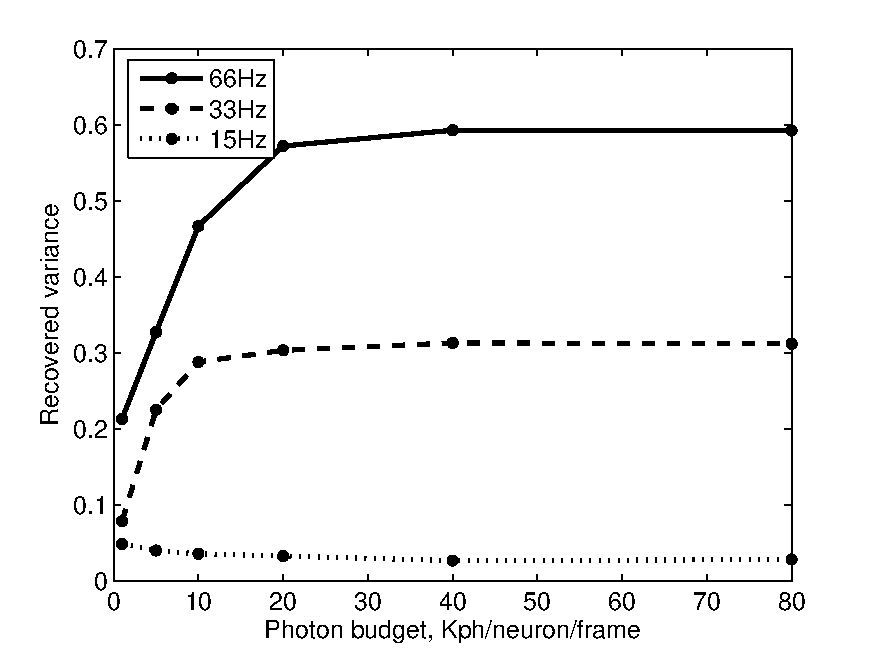
\includegraphics[width=3in]{../figs/FigureA6_recvar_SNR}
\caption{Accuracy of inferred connectivity weights as function of the noise amount in the calcium imaging data, as quantified by experimental photon budget per neuron-frame, for frame rates of 15 Hz, 33 Hz and 66 Hz. Photon counts on the order of 20-40 Kph/frame/neuron are required to achieve the upper bound due by the frame rate. Connectivity matrix here was inferred from simulated fluorescence data using independent approximation algorithm. . Simulation conditions are the same as in Figure \ref{fig:recvar}.}
\label{fig:recvar-SNR}
\end{figure}

\begin{figure}[h]
\centering
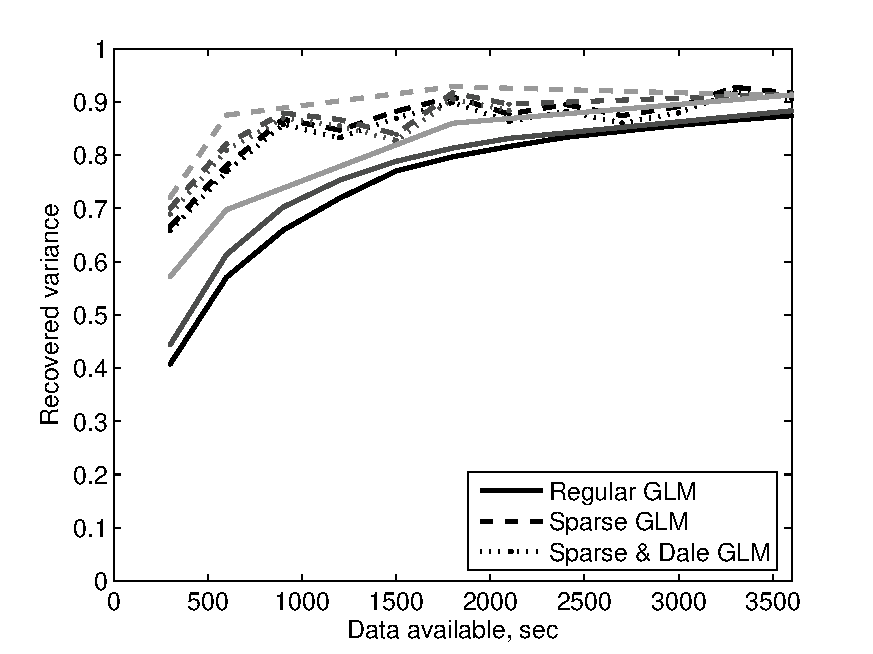
\includegraphics[width=3in]{../figs/FigureA7_recvar_NT}
\caption{Accuracy of inferred connectivity weights as function of the imaging time and neural population size.
Incorporating simple priors such as exponential prior on the connectivity weights allows to boost reconstruction accuracy dramatically (dashed lines). In this latter case, $T=300$ sec is already sufficient to recover 70\% of the variance in the connection weights. Incorporating Dale's prior leads to only marginal improvement (dotted line). As shown in the methods, reconstruction accuracy does not depend on the neural population size $N$.
Here, neural population from $N=10$ to $N=200$ were simulated for different $T$, where
$N=200$ (gray) and $N=100$ (black) are shown. All networks were prepared in similar state by adjusting strength of inhibitory connections to achieve similar mean firing rate $\approx 5$ Hz, although actual firing rate in these networks could vary.
In all cases, $T=5$ min - 0.5 hour is sufficient to produce accurate reconstructions.
}
\label{fig:recvar-NT}
\end{figure}


What minimal conditions for the experimental setup should be met to allow successful reconstruction of the connectivity from calcium imaging data? In Figures \ref{fig:recvar}-\ref{fig:recvar-NT} we answer this question. In Figure \ref{fig:recvar}, the quality of the inferred connectivity matrix is shown as function of the imaging frame rate: imaging frame rates 30-60 Hz are needed to achieve meaningful reconstruction results. These imaging frame rates are feasible for already existing experimental setups. In Figure \ref{fig:recvar-SNR} the quality of the inferred connectivity matrix is shown as function of imaging SNR, as quantified by the photon budget of the experimental setup. From our experience with the analysis of real cells \cite{Vogelstein2009}, the photon budget in real data was $\sim 10$ Kph/cell/frame for in-vivo data collected at 15  Hz and $\sim 100$ Kph/cell/frame for in-vitro data at the same frame rate. As can be seen from Figure \ref{fig:recvar-SNR}, the photon budget necessary for accurate reconstructions was 10-40 Kph/neuron/frame. For lower photon counts the amount of noise in calcium imaging data degraded inferred connectivity matrices significantly.
In Figure \ref{fig:recvar-NT} the quality of the inferred connectivity matrix is shown as function of the calcium imaging data amount from 5 min to 1 hour. The minimal necessary amount of data depended substantially on whether prior information about the distribution of connectivity weights was incorporated into the M-step. In particular, for M-step based on simple GLM, the calcium imaging duration necessary to achieve $r^2$=0.5 for the reconstructed connectivity matrix was $T\sim 10$ min, while for M-step solving sparse-GLM $r^2>0.5$ was achieved already at $T\sim 5$ min (assuming 5 Hz of firing rate).
These numbers appear to be well within limitations of the existing experimental setups.
Furthermore, in agreement with theoretical analysis in the Methods, the accuracy of the reconstruction did not depend on the size of imaged neural population, with the same reconstruction quality observed for the same amount of data for $N=50-200$ neurons. In all cases, good reconstructions were obtained already with $T\sim 5-30$ min of calcium imagign data.


\subsection{Accuracy of the estimates and Fisher information matrix} \label{sec:methods:accuracy_Fisher}

XXX THIS SHOULD PROBABLY BE REDUCED A BIT AND MOVED TO THE RESULTS;
BETTER TO EXPLAIN THE RESULTS AFTER WE ACTUALLY SHOW THEM XXX

To determine the necessary amount of data for accurate estimation of
the functional connectivity matrix, we calculate Fisher information
for $P[\bw| \bX]$. Assuming for simplicity perfect knowledge of spike
trains (i.e. such not corrupted by inference errors from calcium
imaging) and single time-bin coupling, i.e. $h_{j}(t)\neq 0$ only for
time-delay $t=1$, we write the Fisher information matrix as:

\begin{equation}
\begin{array}{rl}
C^{-1}=\frac{\partial (-\ln P)}{\partial \w_{ij}\partial \w_{i'j'}}
=-&\delta_{ii'}\sum\limits_t\left[
n_i(t)n_{j}(t-1)n_{j'}(t-1)\left(-\frac{f'(J_i(t))^2}{f(J_i(t))^2} +
\frac{f''(J_i(t))}{f(J_i(t))}\right) \right. \\
&\left.-\Delta (1-n_i(t))n_{j}(t-1)n_{j'}(t-1)f''(J_i(t))\right].
\end{array}
\end{equation}

 where $f'$ and $f''$ correspond to the first and second derivatives of our linking function (c.f Eq. \ref{eqn:glm:definition}), and $\delta_{ii'}$ is XXX ? XXX.  When $f(J)=\exp(J)$ XXX Y: we don't use an exponential here.  is it worth modifying this accordingly? XXX, and coupling between spikes is week, this may be rewritten as:

\begin{equation}\label{eqn:fisher}
\begin{array}{rl}
C^{-1}
&=\delta_{ii'} (T\Delta) P[n_i(t)=0, n_j(t-1)=1, n_{j'}(t-1)=1]E[f(J_i(t))|n_i(t)=0, n_j(t-1)=1, n_{j'}(t-1)=1] \\
&\sim (T\Delta)\left[(r \tau_w)\delta_{ii'}\delta_{jj'}+O((r \tau_w)^2)\right]r.
\end{array}
\end{equation}

Here $(T\Delta)$ is the total observation time, $ \tau_w$ is ``the coincidence time'' --- the typical EPSP/IPSP time-scale over which the spike of one neuron affects the spike probability of the other neuron --- and $r \approx E[f(J_i(t))|n_i(t)=0, n_j(t-1)=1, n_{j'}(t-1)=1]$ is the typical firing rate.  For successful determination of the functional connectivity matrix $\bw$, the variance $C$ should be smaller than the typical scale $\langle \bw^2\rangle$, i.e.

\begin{equation}
(T\Delta) \sim (\bw^2 r^2  \tau_w)^{-1}.
\end{equation}

For typical values of $\bw^2\approx 0.1$, $r\approx 5$  Hz and $ \tau_w \approx 10$ msec, 
with this order of magnitude estimate we obtain $T$ of the order of hundred seconds. This theoretical estimate of the necessary amount of fluorescent data is in good agreement with our simulations below.

Note also that necessary recording time does not depend on the number of neurons in the imaged network $N$. This unexpected result is the direct consequence of the special form of $C^{-1}$ in Eq. \ref{eqn:fisher}. In particular, when $r \tau_w <<1$, this matrix is dominated by the diagonal term $(T\Delta)(r^2  \tau_w)$, and so the Fisher information matrix is predominantly diagonal with the scale $(r^2 \tau_w T\Delta)^{-1}$, independent of the number of neurons $N$. This theoretical result is also directly confirmed in our simulations below.

\subsection{Impact of using priors on the inference}

\begin{figure}[h]
\centering
\begin{minipage}[c]{0.45\hsize}
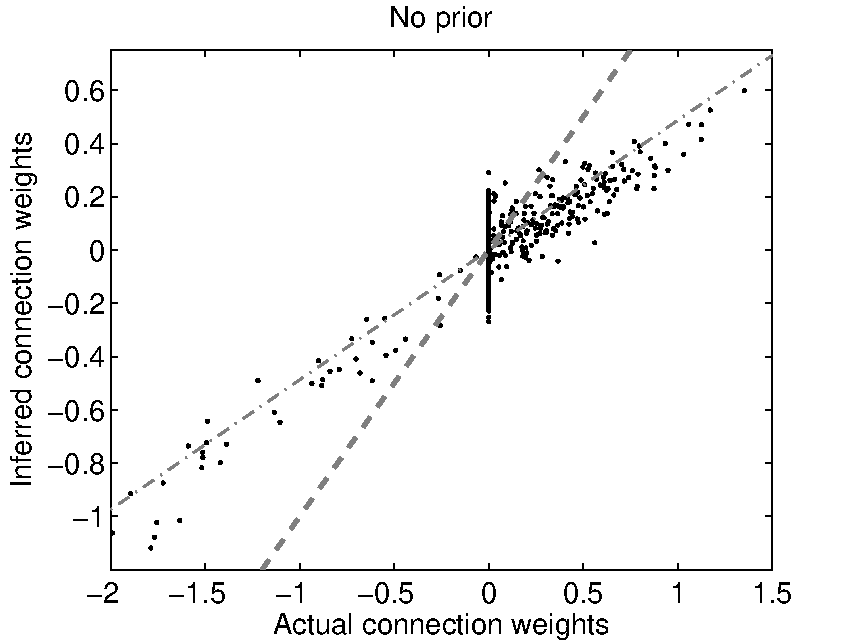
\includegraphics[width=\hsize]{../figs/FigureA10_regular_sol}
\end{minipage}
\begin{minipage}[c]{0.45\hsize}
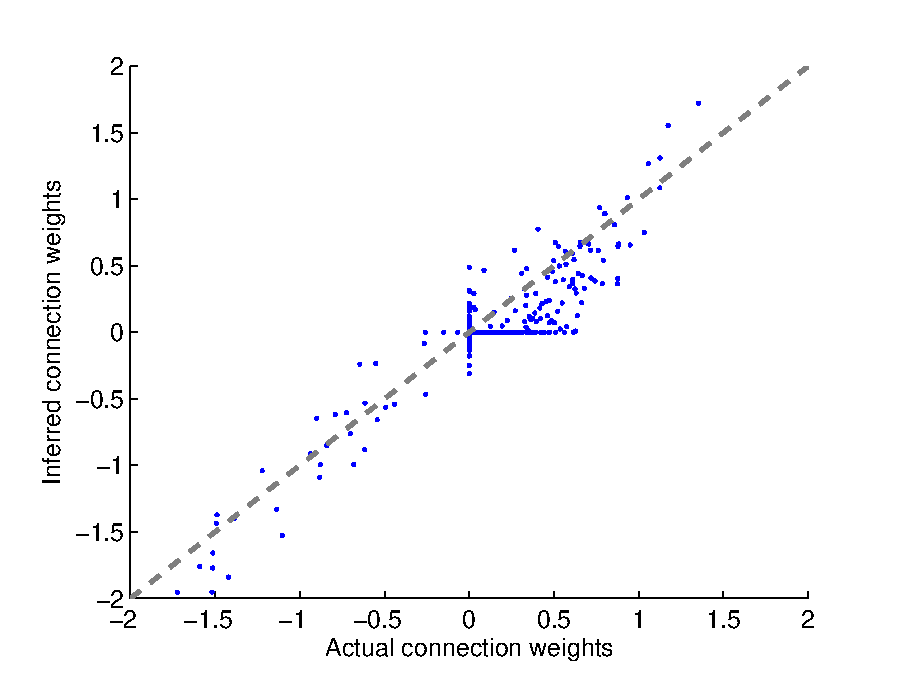
\includegraphics[width=\hsize]{../figs/FigureA10_sparse_sol}
\end{minipage}
\caption{Incorporating simple priors on the distribution of connectivity weights in the Bayesian inference algorithm, such as exponential sparseness prior, is essential to achieve much more accurate reconstructions than using simple GLM from a smaller amount of calcium imaging data. Here, connection weights reconstructed using simple GLM (left panel) or sparse-prior GLM (right panel) are shown in a scatter plot for a network of $N=50$ neurons firing at $\approx 5$ Hz and imaged for $T=600$ sec. $r^2=0.64$ for simple GLM solution and $r^2=0.85$ for sparse-GLM solution.}
\label{fig:sparse}
\end{figure}

\begin{figure}[h]
\centering
\begin{minipage}[c]{0.45\hsize}
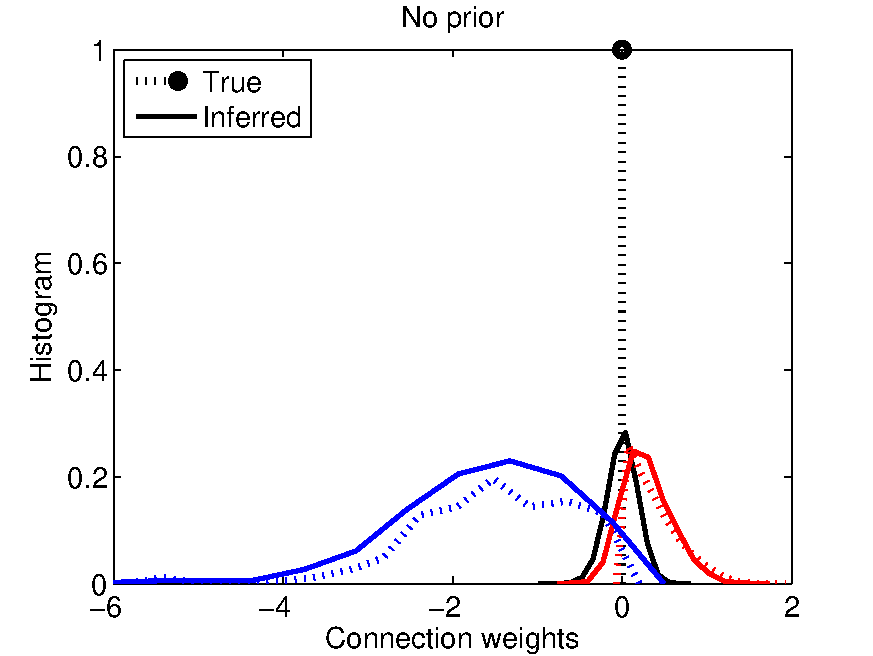
\includegraphics[width=\hsize]{../figs/FigureA3_hist_glm200}
\end{minipage}
\begin{minipage}[c]{0.45\hsize}
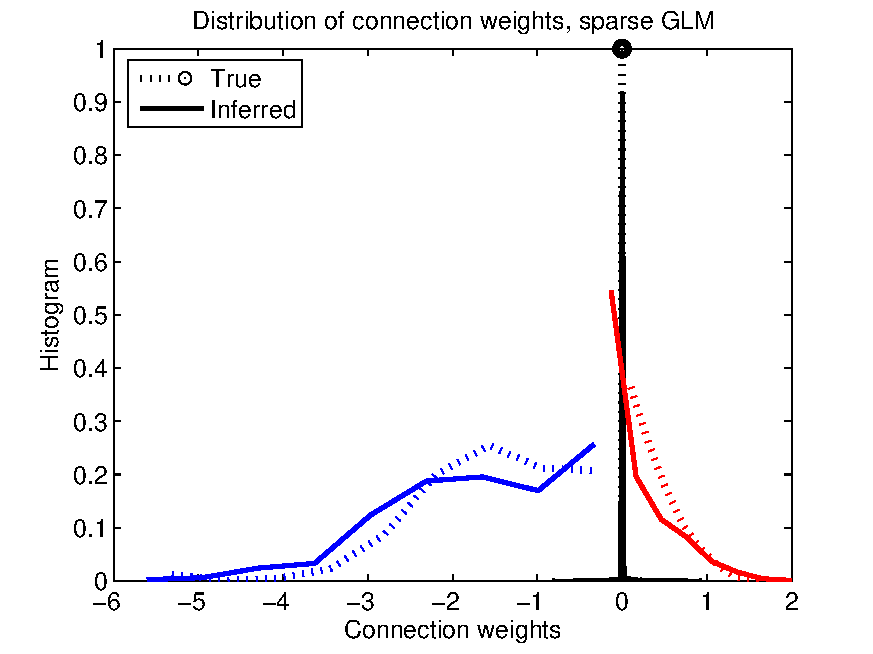
\includegraphics[width=\hsize]{../figs/FigureA3_hist_spa200}
\end{minipage}
\caption{Distribution of inferred connection weights using simple GLM (left) and sparse GLM (right) vs true distributions. When sparse exponential prior on the distribution of connection weights is enacted, dispersion in inferred connection weights is substantially reduced and, in particular, it becomes possible to reliably determine which neural pairs are connected. Distributions are shown for a network of $N=200$ neurons firing at $\approx 5$ Hz and imaged for $T=600$ s was used here.}
\label{fig:distros}
\end{figure}

Taking into account simple prior information about the connectivity matrix resulted in dramatic improvement of the inferred connectivity matrix, Figure \ref{fig:sparse} and \ref{fig:distros}. Sparseness prior resulted in dramatic improvements allowing successful reconstruction from as little as 5 min of calcium imaging data, and allowing to achieve for $T\approx 10$ min the same level of accuracy that would otherwise require up to $T\approx 1$ hour of calcium imaging data, Figure \ref{fig:recvar-NT} and \ref{fig:sparse}. 
Note, however, that sparse prior resulted in added scale bias into obtained connectivity estimate, thus, effectively destroying information about the scale of connection weights in a population.
Furthermore, information about connected neural pairs and about inhibitory or excitatory nature of particular neuron could be reliably obtained, Figure \ref{fig:distros}.
Dale's prior, on the other hand, only led to ~10\% in the correlation coefficient $r^2$ of the reconstructed connectivity matrix, and was not found significant.

\subsection{Impact of strong correlations and deviations from generative model on the inference}

%Fig 7: non-robustness to strong correlations
%top panels: rasters
%bottom panels: corrected scatter plots
%
\begin{figure}[h]
\centering
\begin{minipage}[c]{0.45\hsize}
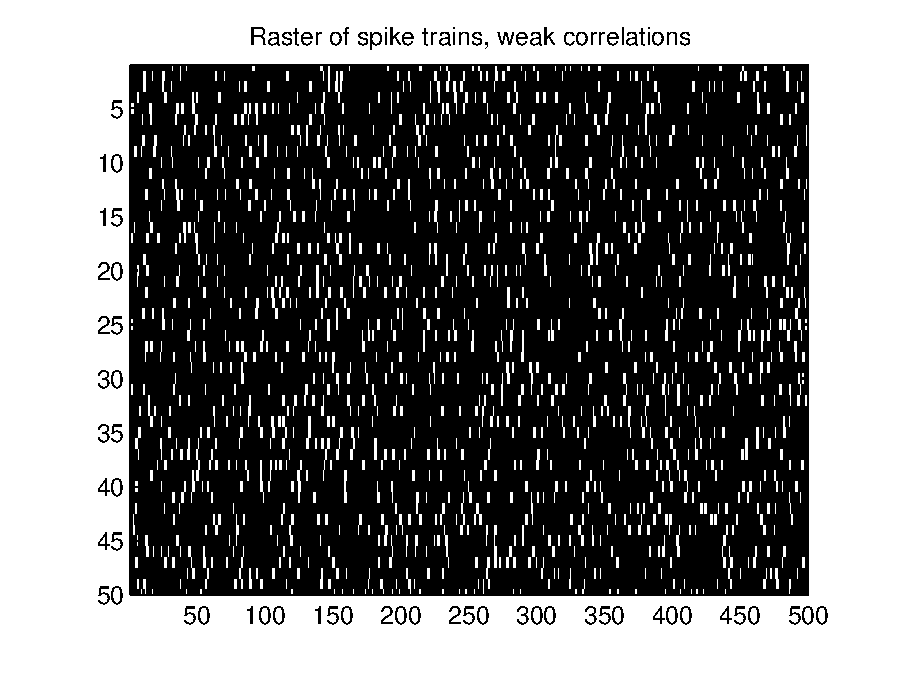
\includegraphics[width=\hsize]{../figs/Figure7b_raster_weak}
\end{minipage}
\begin{minipage}[c]{0.45\hsize}
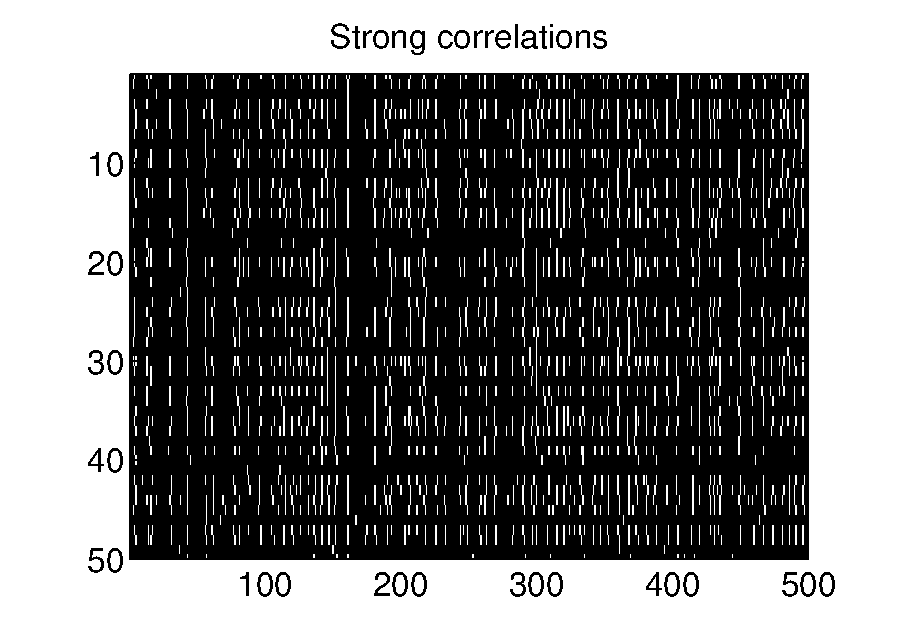
\includegraphics[width=\hsize]{../figs/Figure7a_raster_strong}
\end{minipage}
\begin{minipage}[c]{0.45\hsize}
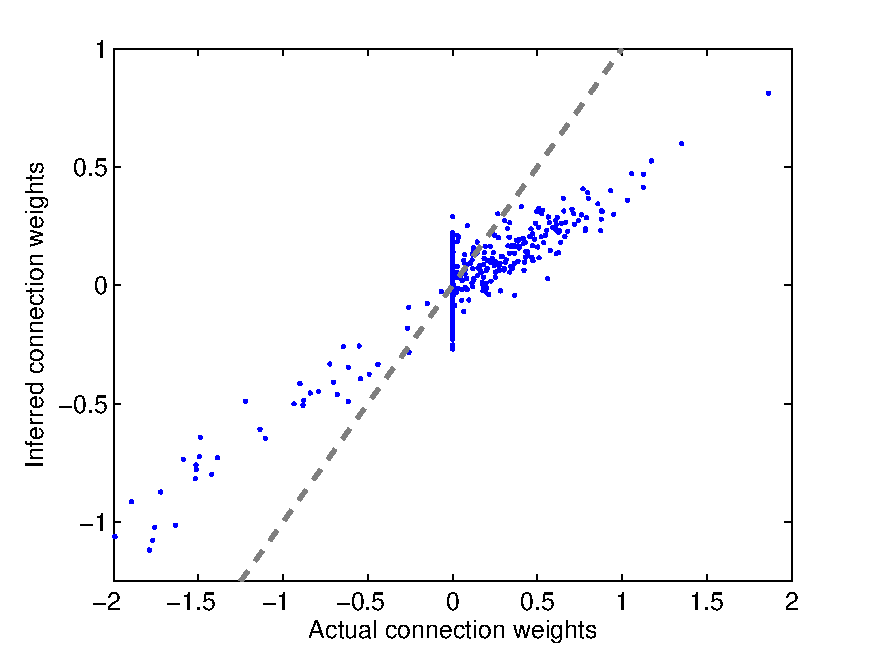
\includegraphics[width=\hsize]{../figs/FigureA8_weak_corr}
\end{minipage}
\begin{minipage}[c]{0.45\hsize}
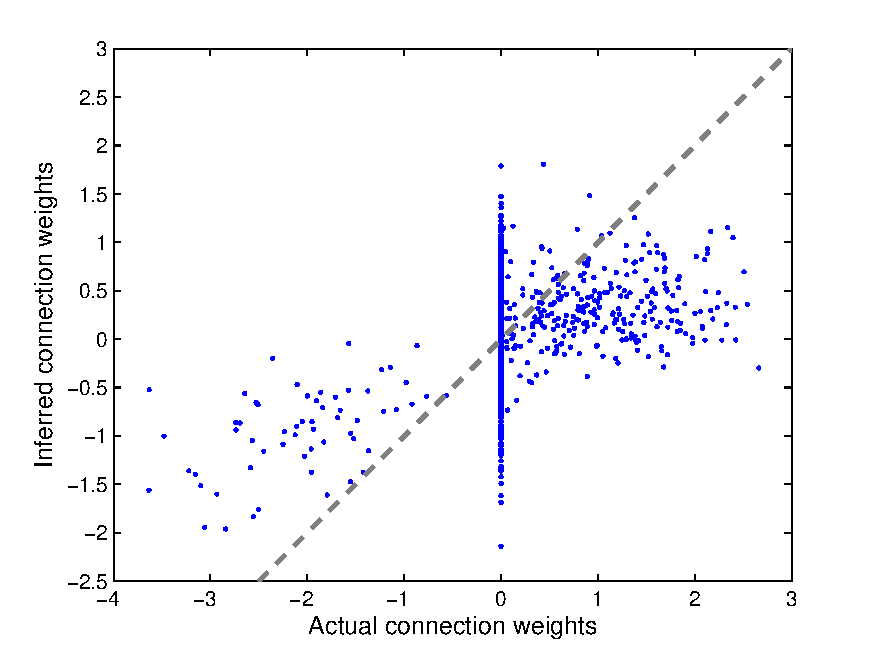
\includegraphics[width=\hsize]{../figs/FigureA8_strong_corr}
\end{minipage}
\caption{
Diverseness of observed neural activity patterns is required for
functional connectivity to give access to the actual ``anatomical'' structure
of the neural circuit. Here, 15 sec of simulated spike trains for a weakly coupled network (upper-left) and a network with strongly coupled component (upper-right) are shown.
In weakly coupled network spikes are sufficiently uncorrelated to give access to all different neural activity patterns needed to properly estimate true weights ${\bf w}_i$. In strongly coupled case, many instances of highly synchronous locked firings are evident, thus preventing observation of sufficiently rich ensemble of activity patterns.
Accordingly, GLM solution for the strongly coupled neural network (lower-right) does not
represent the true connectivity of the circuit, even for the weakly coupled circuit's component. This is contrary to the weakly-coupled network (lower-left) where true connectivity is successfully estimated.
Networks of $N=50$ neurons firing at $\approx 5$ Hz and imaged for $T=600$ sec were used to produce this figure.}
\label{fig:rasters}
\end{figure}

\begin{figure}[h]
\centering
\begin{minipage}[c]{0.45\hsize}
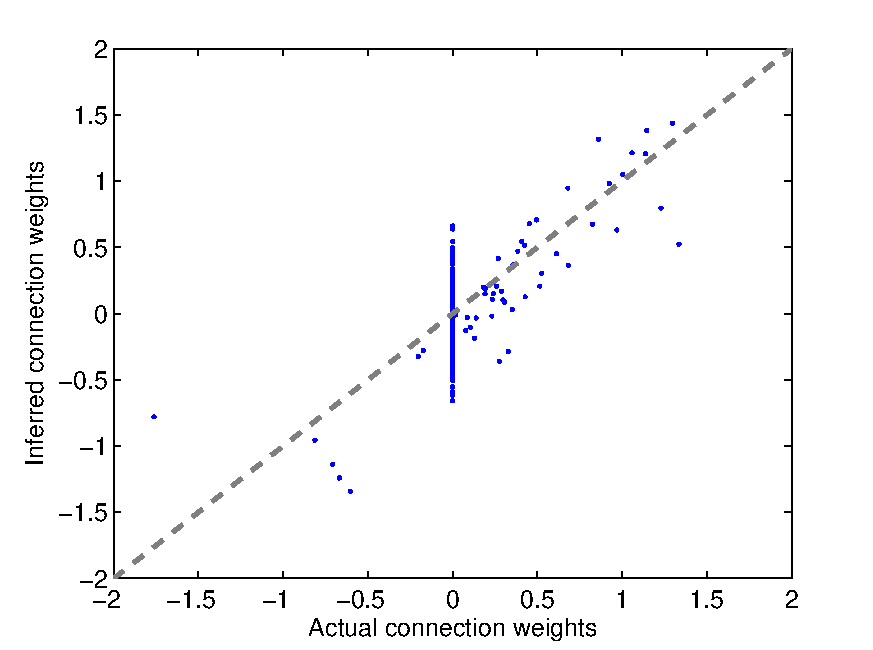
\includegraphics[width=\hsize]{../figs/FigureA9_all_same_sol}
\end{minipage}
\begin{minipage}[c]{0.45\hsize}
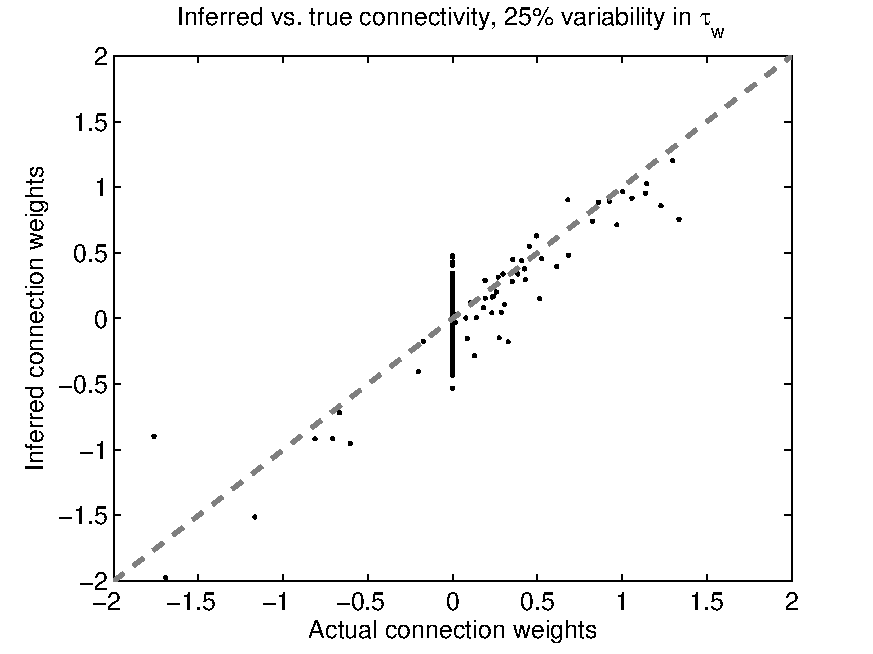
\includegraphics[width=\hsize]{../figs/FigureA9_variable_25}
\end{minipage}
\caption{Bayesian inference algorithm is robust to distortions of the
underlying generative model. One distortion that should be expected is variability of the EPSP time courses from neuron to neuron, and possibly synapse to synapse.
With up to 25\% variability allowed in EPSP time scales $\tau_w$ (right panel) our algorithm provided reconstructions of the same quality as when all $\tau_w$ were the same (left panel). Simulation conditions are the same as in Figure \ref{fig:recvar}.}
\label{fig:vartau}
\end{figure}


``Anatomical'' connectivity was recovered in our experiments despite potential problems noted in the literature [XXX], e.g. such as common input from correlated neurons. This is primarily due to the particular form of the activity in our neural networks, whereas firing of neurons occurred independently, thus, allowing GLM explore the full range of possible input configurations and disentangle common inputs.

Estimation of the functional connectivity is fundamentally routed in observing changes in the spike rate conditioned on the state of the other neurons. Intuitively, such estimation can be compared to observing changes in $p({\bf n}(t))=\exp(\sum_j \w_{ij}n_j(t))$ for different neural configurations ${\bf n}(t)$, i.e. estimating a vector ${\bf w}_i$ from a number of dot-products ${\bf w}_i\cdot {\bf n}(t)$ with different vectors ${\bf n}(t)$. In order to properly estimate all components of ${\bf w}_i$ the set of available ${\bf n}(t)$ should be rich enough to span all $N$ dimensions of ${\bf w}_i$. In case of independent firing such condition is clearly satisfied.  Should this condition be violated, however, e.g. due to high correlation between spiking of few neurons, spike trains may not provide access to the complete vector ${\bf w}_i$, and the connection weights inferred from such activity data may effectively ``aggregate'' true connection weights in arbitrary linear combinations.

We carried out a simulation of hypothetical ``strongly'' coupled  neural network, where in addition to weak sparse connectivity we introduced sparse random strong connectivity component. In some sense, we allowed a fraction of neurons to couple strongly to the other neurons, thus making them ``command'' neurons ``driving'' activity of the other neurons. The strength of strong connectivity component was chosen to build up the actual firing rate dynamically from the baseline rate of $r=\exp(b)\approx 1$ Hz to $\approx 5$  Hz.
Such neural network showed patterns of activity very different from the weakly coupled networks inspected above, Figure \ref{fig:rasters}.  In particular, large number of highly correlated, synchronously locked firings of many neurons were evident in this network.  Likewise, our algorithm was not able to identify the true connectivity matrix correctly, Figure \ref{fig:rasters}.

%Fig 8: robustness to variability in tau_h
%left: corrected scatter plot for (1) assuming same tau's, and (2) assuming they are all diff
%right: distributions of the weights, for truth and the above two approaches
%
%Fig 9: sparse glm improves fit (same format as Fig 8)
%




On the other hand, our inference algorithm showed significant robustness to different deviations from the generative model.
One important deviation that is likely to be present in the real data is variations in the time-scales of EPSPs of different synapses. Up to now, all EPSP time-scales $\tau_w$ were assumed to be the same in our inference algorithm.
Variability in $\tau_w$ would result in added variance in the estimated weights $w_{ij}$ through $\tau_w$ dependence of the scaling factor Eq.(\ref{eqn:bias}).
Still, we found that such added variance to be insignificant in our simulations with $\tau_w$ varying for up to 25\%, Figure \ref{fig:vartau}.


%Fig -: real data
% \begin{figure}[h]
% \centering
% \begin{minipage}[c]{0.45\hsize}
% 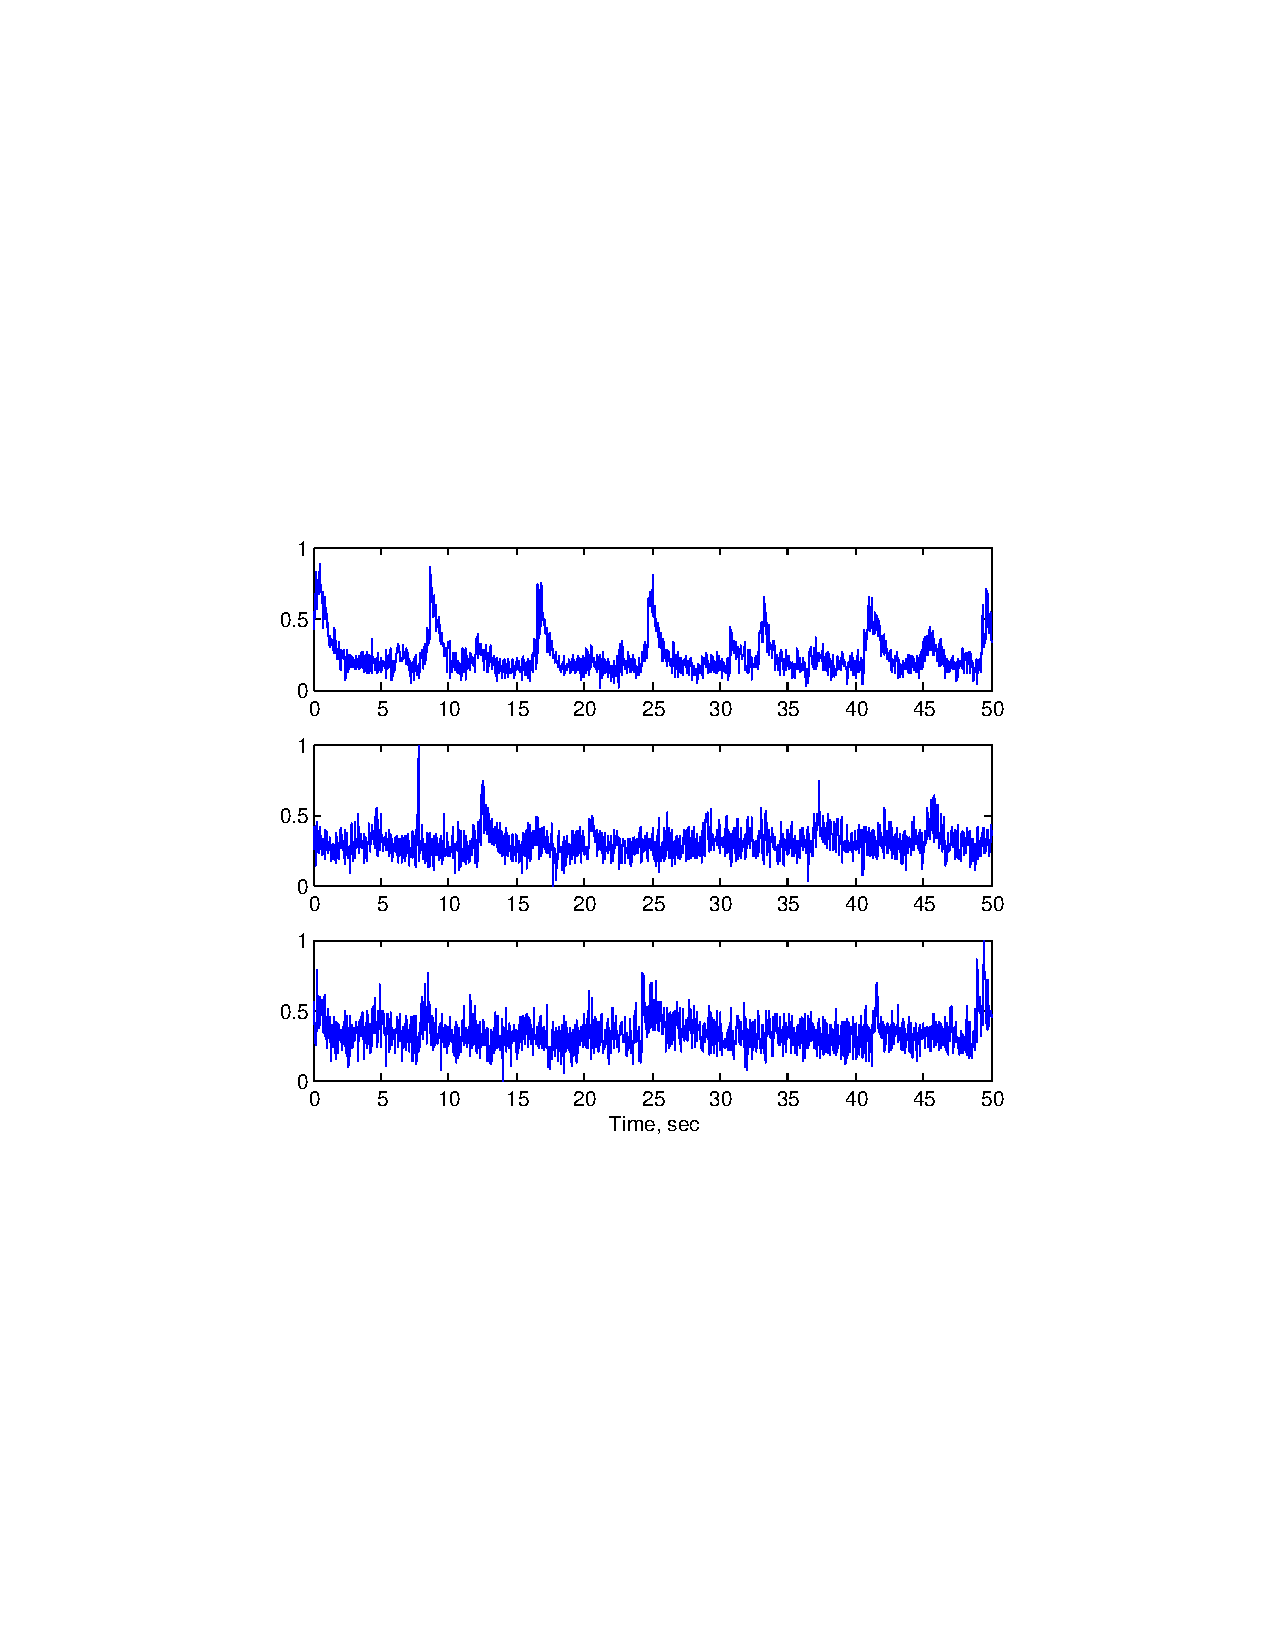
\includegraphics[width=\hsize]{../figs/FigureA11_real_traces}
% \end{minipage}
% \begin{minipage}[c]{0.45\hsize}
% 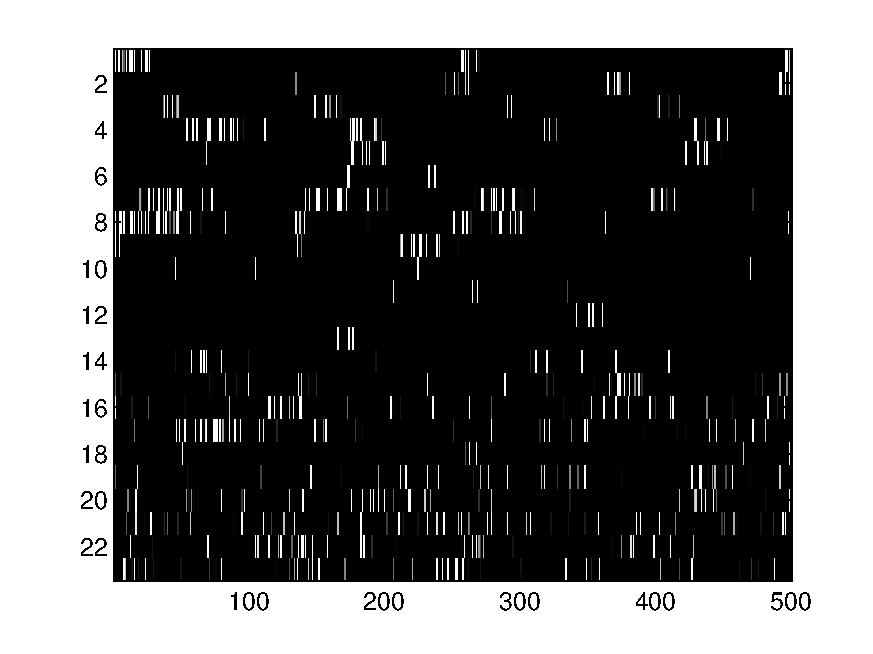
\includegraphics[width=\hsize]{../figs/FigureA11_real_raster}
% \end{minipage}
% \begin{minipage}[c]{0.3\hsize}
% 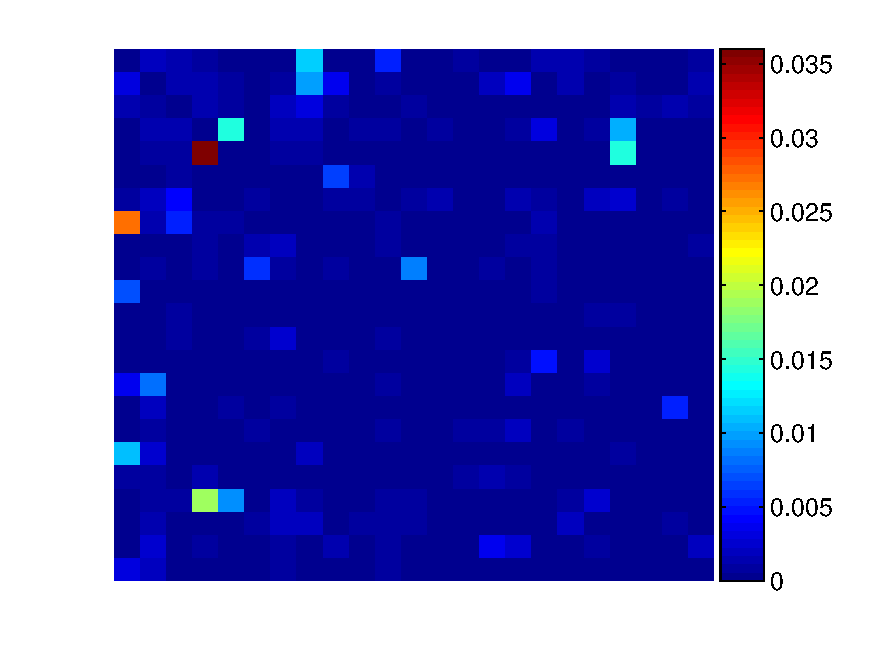
\includegraphics[width=\hsize]{../figs/FigureA11_real_Xcorr}
% \end{minipage}
% \begin{minipage}[c]{0.3\hsize}
% 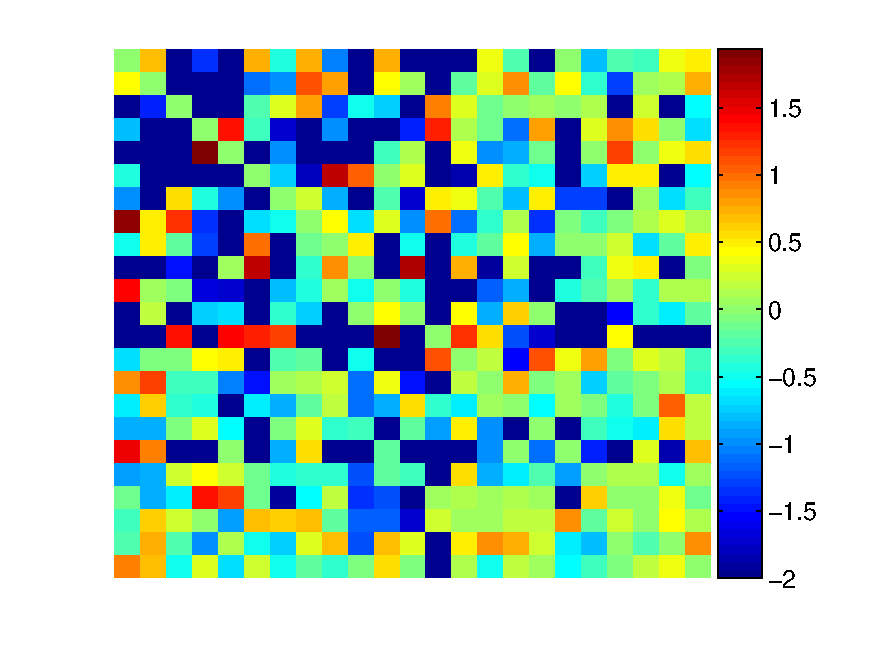
\includegraphics[width=\hsize]{../figs/FigureA11_real_glm}
% \end{minipage}
% \begin{minipage}[c]{0.3\hsize}
% 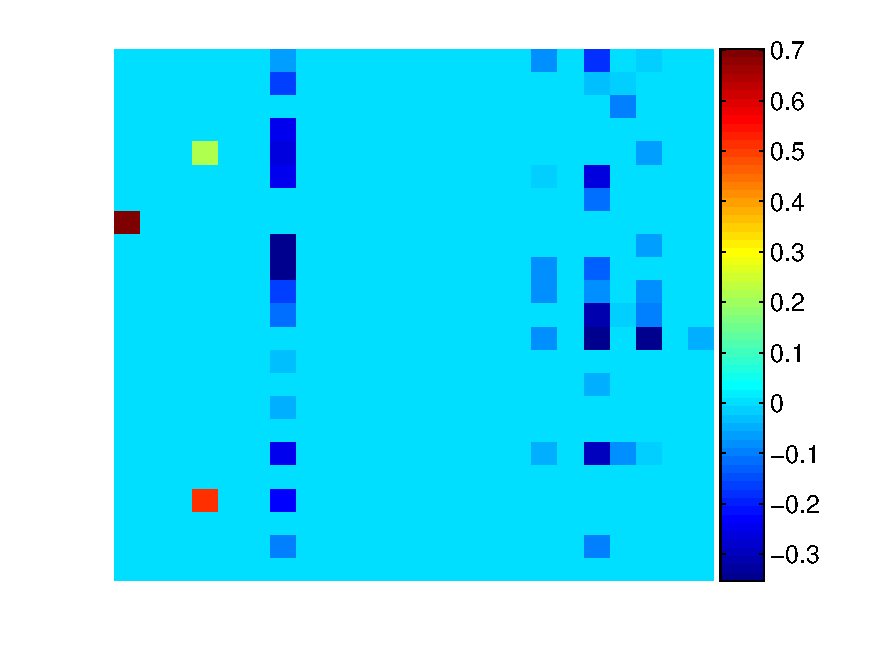
\includegraphics[width=\hsize]{../figs/FigureA11_real_sparse}
% \end{minipage}
% \caption{Functional connectivity matrix inferred from a sample of actual calcium imaging data for $N=72$ cells in [XXX], imaged for $T\approx 260$ sec at 15 Hz.
% $N=23$ neurons with spikes at sufficient SNR were selected, and functional connectivity reconstructed using independent approximation algorithm. Firing cell of these cells was 0.1-1 Hz and 20-200 spikes were collected for each neuron.
% Upper-left panel shows example of actual fluorescence traces from selected cells, best to worst. Upper-right panel shows a raster of inferred spike trains for first 100 sec of imaging data. Lower panels show left-to-right the time-delayed cross-correlation matrix for selected neurons, simple GLM solution and sparse GLM solution, respectively. A consistent connectivity matrix is obtained here, with sparse solution having sparseness of $\approx 10 \%$, and all neurons automatically respecting Dale's law without explicitly enforcing it. Two clearly excitatory, and three clearly inhibitory neurons can be seen, with remaining neurons not showing significant couplings.}
% \label{fig:real}
% \end{figure}


%We applied our algorithm to a sample of the real calcium imaging data from [XXX], totaling about 5 minutes of imaging for a population of 72 cells in [XXX]. Out of these, about 23 cells had fluorescence traces indicative of spikes, while the other cells were either silent or did not shown SNR sufficient for analysis. These 23 cells were selected for futher processing. 20-200 spikes were found for each cell, corresponding to firing rates from 0.07 Hz to 0.8 Hz.
%We then identified functional connectivity matrix for this population. Sparse solution resulted in consistent connectivity matrix with sparseness of about 10\%, automatically respecting Dale's law, and clearly indicating two strongly connected excitatory neurons and few inihibitory neurons. Although this data lacked independent controls necessary to properly evaluate quality of our obtained reconstruction, it does demonstrate that our approach can be successfully applied under real-life condition to analyze functional connectivity of real populations of neurons.
